\documentclass[a4paper]{article}

\usepackage{graphicx}
\usepackage{float}                                              % Required to use [H] in figures.
\usepackage[colorlinks=true, urlcolor=blue]{hyperref}           % For hyperlinks
\usepackage[margin=1.0cm]{geometry}                     % Set the left margin
\usepackage{tabularx}
\graphicspath{{png}}                                            % Set the default path for images.
\DeclareGraphicsExtensions{.png}                                % Only use image files with .png extension.
\linespread{1.30}                                               % Set line-height.

\hbadness=99999  % or any number >=10000
\vbadness=99999  % or any number >=10000

\newenvironment{twocol}
{
    \vspace*{8pt}
    \tabularx{\textwidth}{|l|X|}
    \hline
}
{
    \hline
    \endtabularx
    \vspace*{8pt}
}

\begin{document}

    \title{Currency Engineering}
    \author{Eric Findlay*}
    \date{2022}
    \maketitle

    *The fundamental results presented in this paper are a re-exposition and extension of a series
    of unpublished papers by the physicist Henri D. Rathgeber (1908-1995). See endnotes for details.

    \tableofcontents

    \section{Introduction}

Economic participants drive markets towards equilibrium. This process, however, is contrained by the
technical properties of the currency used. This paper describes these technical properties and shows
how by correctly isolating and controlling previously coupled components effective control of
currency can be achieved that is highly likely to lead to sustained, stable aggregate economic
equilibrium with full-employment. Around 1741 David Hume\cite{hume1741} observed that real economic
conditions were affected by increases in money supply, which he noted was contrary to the notion
that increases in the price as unit of measurement should be independent of the real factors,

\begin{quotation}
\fontsize{8pt}{8pt}

``If we consider any one kingdom by itself, it is evident, that the greater or less plenty of money is
    of no consequence; since the prices of commodities are always proportioned to the plenty of
    money, and a crown in Harry VII.’s time served the same purpose as a pound does at present ...
    It is indeed evident, that money is nothing but the representation of labour and commodities,
    and serves only as a method of rating or estimating them. Where coin is in greater plenty; as a
    greater quantity of it is required to represent the same quantity of goods; it can have no
    effect, either good or bad, taking a nation within itself; any more than it would make an
    alteration on a merchant’s books, if, instead of the Arabian method of notation, which requires
    few characters, he should make use of the Roman, which requires a great many ... \textbf{But
    notwithstanding this conclusion}, which must be allowed just, it is certain, that, since the
    discovery of the mines in America, industry has encreased in all the nations of Europe, except
    in the possessors of those mines; and this may justly be ascribed, amongst other reasons, to the
    encrease of gold and silver.  Accordingly we find, that, in every kingdom, into which money
    begins to flow in greater abundance than formerly, every thing takes a new face: labour and
    industry gain life; the merchant becomes more enterprising, the manufacturer more diligent and
    skilful, and even the farmer follows his plough with greater alacrity and attention. This is not
    easily to be accounted for, if we consider only the influence which a greater abundance of coin
    has in the kingdom itself, by heightening the price of commodities, and obliging every one to
    pay a greater number of these little yellow or white pieces for every thing he purchases.''

\end{quotation}

Hume's considerations suggest that any effective economic model requires an understanding of both
how economic participants interact in the market but also an understanding of the role of money in
those market transactions. A basic supply and demand model infers a macro-economic equilibrium where
aggregate demand and aggregate supply are in equality, or equivalently, that aggregate excess supply
and demand across markets should average out to close to zero. Contrary to this expectation, all
countries experience a sustained state of unemployment and excess aggregate supply as shown in
Figure \ref{fig:ui_all_data}.

\begin{figure}[H]
\centering

\includegraphics[scale=0.48]{blank}
\caption{Inflation Rate vs. Unemployment Data}
\label{fig:ui_all_data}
\end{figure}

Given that any currency mechanism is absent from this model of supply and demand and that Hume's
observations suggest currencies have significant effects, it seems reasonable to find a way to
include currency in our model. This leads to the question of what methods should be used to analyze
the properties of currency. Because currency is at its essence a information structure the way to
approach this problem is the same way as other similar systems, an example being the internet, as an
engineering problem, and in particularly as a problem of the engineering and control of dynamic
systems. Economic theory approaches economic problems similarly to the way medicine treats the human
body, by applying relatively small changes, such as medicine, in response to various pathologies.
Destructuring and rebuilding biological systems is impossible. Importantly however, the control
system for economies, the currency, can indeed be destructured and rebuilt from first principles.
Thus we take a different approach, viewing currency more like a robotics problem, something that can
be built from the bottom up. In general a currency is a set of accounts, eaching holding a number
that can be transfered to other accounts, but we require a more concrete formulation of how economic
participants \textit{use} the currency, and so we categorize the way a currency is used into
different transaction types.  and these can be categorized into various types of transactions. We
categorize the most common transactions into exchange transactions, time transactions, contract
transactions and external transactions.

\begin{figure}[H]
\centering
\includegraphics[scale=0.60]{01_introduction/png/exchange_transaction}
\caption{Exchange Transaction}
\label{fig:exchange_transaction1}
\end{figure}

An exchange transaction is a payment in return goods and services that occurs at one
point in time.

\begin{figure}[H]
\centering
\includegraphics[scale=0.60]{01_introduction/png/time_transaction}
\caption{Time Transaction}
\label{fig:time_transaction1}
\end{figure}

A time transaction extends an exchange transaction and involves the lending of currency at $t_0$.
This money is then used by the borrower for an exchange transaction and a contractural obligation is
established to the lender. At time $t_1$ the principal and interest is repaid to the lender.

\begin{figure}[H]
\centering
\includegraphics[scale=0.60]{01_introduction/png/contract_transaction}
\caption{Contract Transactions}
\label{fig:contract_transaction1}
\end{figure}

A contract transaction extends a time transaction and involves payment for a change in the status or
ownership of a contractural obligation. We also consider external transactions between two
currencies and other types of transactions.

Feedback regulators are self-adjusting mechanisms that work to achieve some desired conditions in
the plant by taking measurements from the plant and feeding back the deviation between the measured
values and the desired set point back into the plant.

\begin{figure}[H]
\centering
\includegraphics[scale=0.60]{01_introduction/png/feedback_schema}
\caption{Feedback Schema}
\label{fig:feedback_schema1}
\end{figure}

We represent the economy as a feedback regulator where the control variables adjusts money supply.
Economic participants then interact by using the currency to make transactions. 

\begin{figure}[H]
\centering
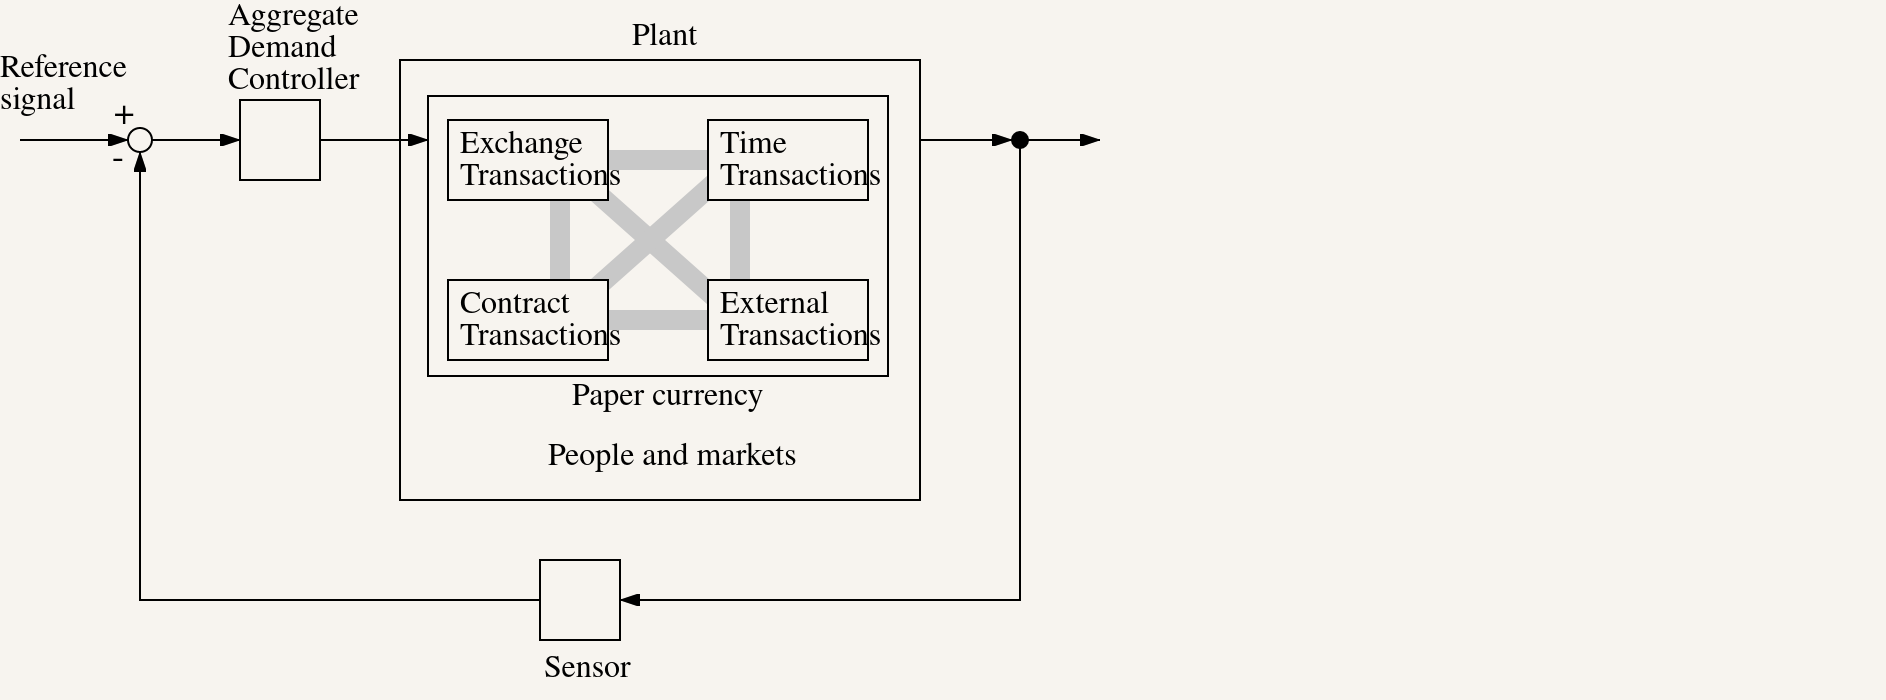
\includegraphics[scale=0.60]{01_introduction/png/economic_feedback_schema}
\caption{Economic Feedback Schema}
\label{fig:economic_feedback_schema1}
\end{figure}

Engineering method is applied to the the currency mechanism not the behaviour of people. The only
assumption about the behaviour of economic participants is that they drive markets to equilibrium.
Our general approach is to take a pared-down version of Figure \ref{fig:economic_feedback_schema1}
and step-by-step introduce each transaction type into the model, and then apply normal engineering
analytical methods. We find that

1. Aggregate demand must be continuously increasing at a rate sufficient to compensate for errors.
Without this requirement the currency constrains the space of possible transactions, preventing
people from driving markets to macro-economic equilibrium.

2. All units written into contracts must be independent of the price level. Without this condition a
positive-feedback instability can result in runaway behaviour under increases in the inflation rate.

3. Contract transactions must be prevented. Without this condition contract transactions can result
in runaway behaviour in prices and difficulties in controlling an overly complex system. Preventing
contract transactions allows for a currency design with precise control over aggregate demand.

A currency that implements these properties is highly likely to result in a economy with sustained
stable aggregate equilibrium and full-employment.


    \section{Introduction to Dynamic Systems and Control}
\label{sec:dynamic_systems_and_control}

TODO

% In this section we introduce the background knowledge and intuitions for the kind of reasoning used
% in later sections.
% 
% \subsection{Negative Feedback}
% 
% \subsection{Positive Feedback}
% 
% \subsection{History of Feedback Control} 
% 
% \subsection{Units}
% 
% \subsection{The Internet}
% 
% \subsection{Micro and Macro}
% 
% \subsection{Dynamic Systems and Discrete Time}
% 
% \subsection{How Feedback Control Goes Wrong}
% 
% \subsection{PID Controllers}
% 
% \subsection{Controllability and Degrees of Freedom}
% 
% \subsection{Errors}
% 
% \subsection{Safety and Liveness}
% 
% \subsection{Control System Design}
% 
% \subsection{System Specification}
% \label{sec:system_specification}
% 
% \subsection{Brief History of Mechanic Feedback Mechanisms}
% 
% Prior to the Wright brother's first flight in December 1903, Orville and Wilbur Wright believed that
% the most fundamental problems they needed to solve were control problems. In September 1901 Wilbur
% Wright's first public presentation on the feasibility of heavier-than-air flight stated that ``When
% this one feature [control] has been worked out the age of flying machines will have arrived, for all
% other difficulties are of minor importance."\cite{wright1908}
% 
% \subsection{Feedback}
% 
% \underline{feedforward}
% 
% \underline{negative feedback}
% 
% \underline{positive feedback}
% 
% \subsection{PID Controllers}
% 
% PID controllers are very simple. PID controllers are remarkably robust and in universal use for a
% great variety of feedback control. So while they are not the only solution, they are a good starting
% model for thinking about feedback systems.
% 
% \underline{History}
% 
% TODO: Huygens
% 
% TODO: Watt
% 
% TODO: Maxwell
% 
% (around 1912)
% 
% Elmer Sperry, who introduced the gyroscope invented by TODO to the USA, developed various automatic
% steering systems.
% 
% \begin{quote}
% Elmer Sperry realized that the performance of the gyropilot seemed uncanny, for he had been told
% that no one could possibly invent a device incorporating the intuition of an expert quartermaster.
% He had in fact analyszed the "intuition" problem when he first began work on the pilot in 1912 and
% had decided that the helmsman's intuition was, in essence, tha ability to "ease off" and "meet" the
% helm.[21] Easing off involved lessening the rudder angle after the rudder had been put over and the
% ship had responded by swinging toward the desired heading; meeting was putting the rudder over to
% the other side (overthrow) to counter the tendency of the ship's angular momentum to carry it past
% the desired heading. If the helmsman did not perform these functions with skill, the ship continued
% to yaw. Sperry set out to devise a way of performing these functions mechanically and automatically.[22]
% \end{quote}
% 
% `Easing off' is `Meeting' take the role of the `D' component of a PID controller, where the
% controller responds to the \textit{rate} at which the plant is moving towards the set point.
% 
% TODO: Integral?
% 
% 
% \subsection{How Feedback Systems Go Wrong}
% 
% \underline{Wrong Model}
% 
% \underline{Complexity}
% 
% \underline{Delay}
% 
% \underline{Not Smooth}
% 
% \underline{Errors}
% 
% 
% \underline{Wrong Parameters}
% 
% While we introduced PID controllers in some detail, we don't consider their application to our
% problem in detail. Th The general notion of feedback is critical to our model. To deepen our
% understanding of feedback controllers. The reason why contemporary economies are unstable and
% sub-optimal, running at high levels of unemployment is because we have the wrong model. Before the
% practical application of PID controllers to currency control systems, we must find a better model. 
% 
% \subsection{Errors and Noise}
% 
% \subsection{Internet}
% 
% % Some Abstractions - Multiplexing
% % Packet Switching
% % Some Abstractions - Hiding
% 
% \underline{Introduction}
% 
% \underline{TCP/IP}
% 
% \underline{Congestion}
% 
% \underline{Routing}
% 
% % We are looking for a way that we can keep the conditions of the system in some desirable state.
% % Examples are ... If the system is predictable can use an open system. Many systems, however are not
% % completely predictable. In many case, despite the unpredictability we can still control the system
% % to a certain degree. One method is to use a closed system. Another method is to introduce a
% % sophisticated controller into the loop, such as a human, in combination with the mechanism. Examples
% % are ...
% % 
% % A heater with a fixed output.
% % 
% % A heater with a thermostat.
% % 
% % Using a schema similar to \ref{fig:feedback_schema} we can represent the cyclist as,
% % 
% % \begin{figure}[H]
% % \centering
% % 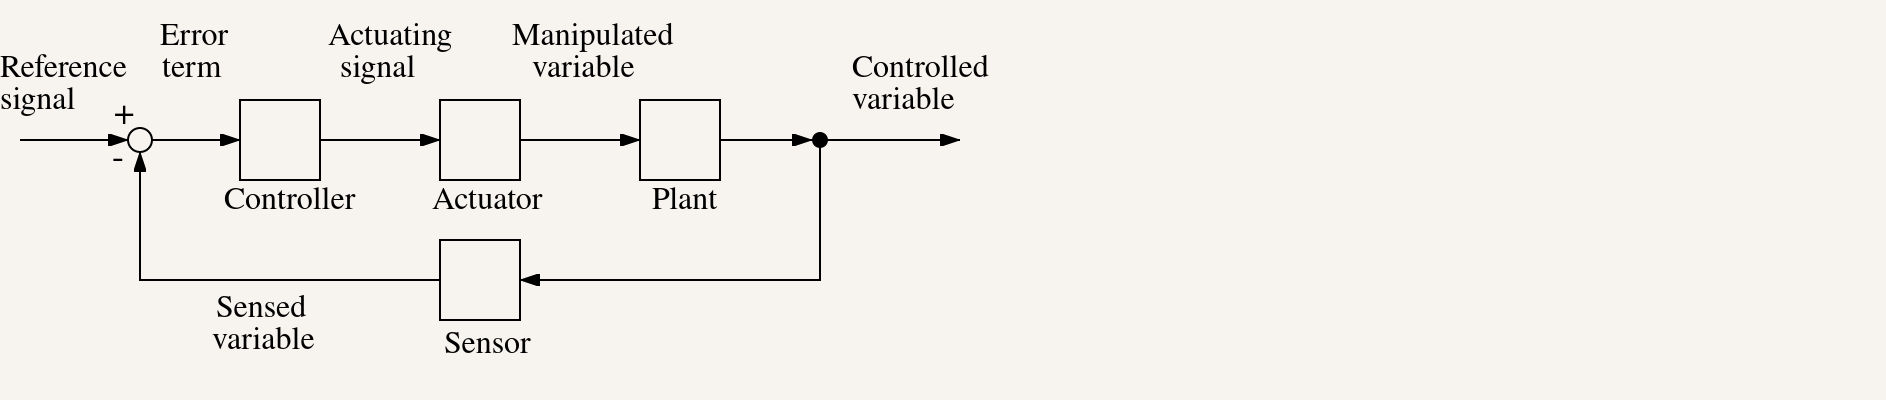
\includegraphics[scale=0.48]{02_dynamic_systems_and_control/png/bicycle_feedback_schema}
% % \caption{Bicycle Feedback Schema}
% % \label{fig:bicycle_feedback_schema}
% % \end{figure}
% % 
% % The 'reference signal' or 'set point' is the goal of the system, in this case most likely a
% % desination and when they want to arrive. The controller takes the set point and the present
% % conditions, i.e. where the cyclist is currently, the location of obstacles, if the road is heading
% % uphill or downhill etc.  weather conditions are, how much time they have remaining and convert this
% % into a control signal. Part of the control signal in this case is observable - the person's
% % adjustments to the handle-bars, other signals are not observable such as decisions on how hard to
% % pedal. The actuator in this case is the cyclists leg muscles, which convert those desicions, and use
% % energy to convert them into pedal pressure. The cyclist then observes the situation again and reacts
% % to the situation by feeding their sensory data back into the 'controller' and so on in a closed
% % loop. In the case of the cyclist we depend on continuous inputs in a changing, often unpredictable
% % environment to adjust behaviour - we require a closed loop system.
% % 
% % \subsubsection{Huygens}
% % 
% % \subsubsection{Watt}
% % 
% % \subsection{PID controller}
% % 
% % \subsubsection{James Clerk Maxwell}
% % 
% % \subsubsection{The Wright Brothers}
% % 
% % Prior to the Wright brother's first flight in December 1903, Orville and Wilbur Wright believed that
% % the most fundamental problems they needed to solve were control problems. In September 1901 Wilbur
% % Wright's first public presentation on the feasibility of heavier-than-air flight stated that ``When
% % this one feature [control] has been worked out the age of flying machines will have arrived, for all
% % other difficulties are of minor importance."\cite{wright1908}
% % 
% % % TODO - this paragraph requires work.
% % 
% % The general view prior to the Wright brothers was that aircraft required the mechanism to
% % self-stabilize. [this was a problem because incorporating stability into the air-craft was at the
% % cost of agility. Possibly because the Wright brothers were bicycle-shop owners, and were aware that
% % bicycles are fundamentally unstable and require human intervention to stay upright, they understood
% % that this control could be done by the pilot rather than the plane.
% % 
% % \subsubsection{Elmer Sperry}
% % 
% % Elmer Sperry was the first to construct a PID controller. One notable characteristic of PID
% % controllers is that despite much work in the design of more sophisticated controllers, PID
% % controllers are by far the most widely used, demonstrating robustness to solve a broad range of
% % control problems.
% % 
% % Elmer Sperry is best known for his construction and application of gyroscopes following the
% % invention of the first practical gyroscope by Hermann Anschütz-Kaempfe in 1904. One of Sperry's
% % applications was the use of a gyroscope as a component in a control system to self-stabilize
% % airplanes.
% % 
% % [longer flights]
% %  
% % Following on from these experiences, he worked with the U.S. Navy to use gyroscopes for stabilizing
% % ships, and then also to build control systems as auto-pilots of ships. Because the control process
% % involved in steering large ships with significant lags and so was relative slow and visible, he was
% % able to observe that skilled helmsmen used a more nuanced 'algorithm' than just a proportional
% % response, and that the helmsman with put the helm over in the opposite to the directions in which
% % the ship was yawing a significantly in advance (a D response), and that helmsman worked the ship
% % upwards in response to currents and prevailing wind (an I response). Sperry then incorporated these
% % three responses (P, I and D) into his mechanical control mechanism which connected the gyroscope to
% % the ships steering.
% % 
% % In 1922 Nicolas Minorsky published a paper which encapsulated the P, I and D into an
% % equation.\cite{minorsky1922}
% % 
% % % chapter:          Dynamic Systems
% % % sec:          Positive Feedback
% % \section{Positive Feedback}
% % 
% % % chapter:          Dynamic Systems
% % % sec:          Error Correction
% % \section{Error Correction}
% % 
% % % chapter:          Dynamic Systems
% % % sec:          Isolation 
% % \section{Isolation}
% % 
% % % chapter:          Dynamic Systems
% % % sec:          Stability
% % \section{Stability}
% % 
% % % chapter:          Dynamic Systems
% % % section:          Internet
% % \section{Internet}
% % 
% % % chapter:          Dynamic Systems
% % % section:          Internet
% % % subsection:       The Network 
% % \subsection{The Network}
% % 
% % The most notable difference between digital networks and the precursor to digital networks - the
% % telephone network - was the notion of packet switching.
% % 
% % % Baran
% % 
% % In the mid 1960s Paul Baran was working on the problem of fault-tolerant networks\cite{baran1964intro}.
% % 
% % \begin{quote}
% % Packet switching technology was not really an invention, but a reapplication of the basic
% %     dynamic-allocation techniques used for over a century by the mail, telegraph, and torn paper
% %     tape switching systems. \cite{roberts1978}
% % \end{quote}
% % 
% % % Pre-allocation
% % 
% % radio, telephony
% % 
% % Analog telephone systems work by setting up a connection between two telephones. This connection
% % takes complete ownership of the physical connection, the wire. Baran proposed to share the physical
% % wire between many connections. Time division multiplexing had been used since the late 19th century
% % to share a single wire to send multiple telegraph messages synchronously. This was called time
% % division multiplexing. The idea was to share the wire by allocating divisions of time for each
% % message. Baran's idea was rather than to multiplex by time, to multiplex by a standardized message
% % block, later termed a 'packet'.
% % 
% % % Dynamic allocation
% % 
% % telegraph and mail systems
% % 
% % \begin{quote}
% % Time division multiplexing appears so natural to data transmission that we might wish to consider an
% % alternative approach -- a standardized message block as a network interface standard.\cite{baran1964intro}
% % \end{quote}
% % 
% % The reasons were
% % 
% % % Efficiency
% % 
% % telephone systems multiplex, i.e. chop up and share out communication by pre-allocating transmission
% % bandwidth a connect (or telephone call). Data transmission comes in short bursts, so the complete
% % physical connection is 'blocked' by the empty parts in a transmission, and so roughly 90 percent of
% % capacity was wasted. We can see why telegraphy was so much cheaper than voice communication. By
% % reducing the granularity of the chopping-up into small packets, one could more efficiently share out
% % the resource, by filling up the blank spaces by some other communication.
% % 
% % % Reliability
% % 
% % % Dynamics
% % 
% % A telephone call fixes the relationship between transmitted information and the network. By
% % packaging up information and assigning each package a destination address, a degree of freedom is
% % introduced between the transmitted information and the network. This means that information can be
% % rerouted, i.e. respond to network conditions, directly attacking the problem of network fault
% % tolerance. We have introduced a negative feedback here, i.e. a response to failure in the network,
% % so as to maintain a stable condition i.e. the success rate of transmissions. We'll look at how this
% % is implemented in section A.
% % 
% % Such dynamic systems require feedback for regulation.
% % 
% % % chapter:          Dynamic Systems
% % % section:          Internet
% % % subsection:       Introduction
% % % subsubsection:    Some Abstractions - Hiding 
% % \subsubsection{Some Abstractions - Hiding}
% % 
% % % TODO: Need a 'hindsight' qualification.
% % 
% % % chapter:          Dynamic Systems
% % % section:          Internet
% % % subsection:       Introduction
% % % subsubsection:    Some Constraints - Distributed Systems 
% % \subsubsection{Some Constraints - Distributed Systems}
% % 
% % \subsubsection{Some Constraints - Burstiness}
% % 
% % \subsubsection{Some Constraints - Heterogenous Networks and Hardware}
% % 
% % In the early 1970s a protocol for joining together many networks. The question is why would you
% % join together networks, each with their own hardware and protocols? Why not select a uniform
% % protocol that is universal across all networks?
% % 
% % \begin{quote}
% %     Even though many different and complex problems must be solved in the design of an individual
% %     packet switching network, these problems are manifestly compounded when dissimilar networks are
% %     interconnected. Issues arise which may have no direct counterpart in an individual network and
% %     which strongly influence the way in which internetwork communication can take place.
% %     \cite{cerf1974}
% % \end{quote}
% % 
% % % TODO: Answer this question
% % 
% % % This section should probably be shifted to a later section.
% % 
% % The main problem of building a network of networks, i.e. the internet was to figure out a way for
% % many different kinds of networks to interoperate. In the foundational paper outlining how to
% % approach this problem\cite{cerf1974}, Cerf and Kahn utilize the hiding abstraction as much as
% % possible, to reduce the complexity of interactions between the different networks. In the abstract
% % they enumerate the functionality to be passed off to individual networks, 
% % 
% % \begin{quote}
% % The protocol provides for variation in individual network packet sizes, transmission failures,
% % sequencing, flow control, end-to-end error checking, and the creation and destruction of logical
% % process-to-process connections.
% % \end{quote}
% % 
% % This could be summarized as passing off dynamic feedback to the individual networks, and specifying
% % the minimum static properties that all networks must share. 
% % 
% % 
% % % Re-check this quote - it might be out of context.
% % \begin{quote}
% %     [Systems] such as real-time traffic that can adapt its sending rate to reduce loss and/or delay
% %     [are] most effective when the adaption occurs on timescales of a single Round-Trip Time (RTT) or
% %     a small number of RTTs, for elastic traffic.\cite{rfc7567}, page 6.
% % \end{quote}
% % 
% % \subsection{Feedback Control Problems of a Packet Switching Network}
% % 
% % To regulate dynamic state, timely and accurate measurement of the right variables are required, to
% % determine the error that is to be fed back into the system.
% % 
% % The two main dynamic processes in the transmission of packets across a network are regulating the
% % routes that are taken across the network and regulating the degree to which links and nodes in the
% % network are filled with packets.
% % 
% % There are several problems specific to the internet that must be solved to do this.
% % 
% % \subsubsection{The Problem of Distributed Systems}
% % 
% % The internet is a distributed system. In a feedback system we require constant feedback of
% % information about the network conditions or the success/faiure of a packet reaching its destination.
% % Because the internet is a distributed system, there is a significant time delay between the actual
% % state of the internet, and the time the sender receives this information. 
% % 
% % Kleinrock\cite{kleinrock 1978}
% % 
% % \begin{quote}
% %     Furthermore, the control of these processes in the time-sharing environment can be very tightly
% %     coupled if desired or left loosely coupled due to the difficulty of tightening the control
% %     between them (indeed, the inherent delay due to the finite speed of light is a fundamental
% %     limitation on the tight coupling of remote processes.
% % \end{quote}
% % 
% % Kleinrock descibes some difficulties in measurement\cite{kleinrock1978},
% % 
% % \begin{quote}
% %     The astute reader will observe that the resource sharing problem stated above sounds very much
% %     like the problem faced in the design of time sharing systems. Surely, with time sharing, we are
% %     faced with the problem of sharing resources among asynchronous processes which behave in a
% %     bursty fashion. The major difference between the two problems, however, is that our problem
% %     exists in a \emph{geographically distributed} environment which requires expensive
% %     communications and coordination functions.
% % \end{quote}
% % 
% % \subsubsection{The Problem of Bursty Data}
% % 
% % The nature of transmission of data is bursty. This feedback response is noisy. To understand the
% % conditions of the network we need to collect data over a sufficient period of time to smooth out the
% % response to an average, which creates further lag.
% % 
% % % TODO: Other reasons burstiness can be a problem:
% % 
% % \begin{quote}
% % The naive assumption might be that there is a simple trade-off between delay and throughput, and
% % that the recommendation that queues be maintained in a "non-full" state essentially translates
% % to a recommendation that low end-to-end delay is more important than high throughput. However,
% % this does not take into account the critical role that packet bursts play in Internet
% % performance. For example, even though TCP constrains the congenstion window of a flow, packets
% % often arrive at network devices in bursts [Leland94]. If the queue is full or almost full, an
% % arriving burst will cause multiple packets to be dropped from the same flow. Bursts of loss can
% % result in a gloabl synchronization of flows throttling back, followed by a sustained period of
% % lowered link utilixzation, reducing overall throughput. \cite{rfc7567} page 8.
% % \end{quote}
% % 
% % \subsubsection{The Problem of Separate Administrative Zones}
% % 
% % % TODO: administration 
% % 
% % \subsubsection{The Problem of Heterogeneous Networks}
% % 
% % % TODO: heterogenouse
% % 
% % \subsubsection{The Problem of Time-outs}
% % 
% % Distributed systems typically use time-outs to collect information about which components in the
% % system are working. Time-outs rely on failure. But in feedback systems we want an earlier response.
% % 
% % % TODO: diagram here
% % 
% % % TODO: History of "Tail-Drop" Queueing
% % 
% % \begin{quote}
% % The traditional technique for managing the queue length in a network device is to set a maximum
% %     length (in terms of packets) for each queue, accept packets for the queue until the maximum
% %     length is reached, then reject (drop) subsequent income packets until the queue decreases
% %     because a packet from the queu has been transmitted. This technique is known as "tail drop",
% %     since the packet that arrived most recently (i.e. the one on the tail of the queue) is dropped
% %     when the queue is full. This method has served the Internet well for years, but it has four
% %     imporant drawbacks. \cite{rfc7567} p. 8.
% % \end{quote}
% % 
% % The first being,
% % 
% % \begin{quote}
% % The "tail drop" discipline allows queues to maintain a full (or almost full) status for long periods
% % of time, since tail drop signals congestion (via a packet drop) only when the queue has become
% % full. It is important to reduce the steady-state queue size, and this is perhaps the most
% % important goal for queue management. \cite{rfc7567} p. 8.
% % \end{quote}
% % 
% % % TODO: This is fifty-years!! after this algorithm was first written.
% % % TODO: When did the term "tail drop" appear?
% % % TODO: Trace back these RFCs.
% % 
% % Jacobson \cite{jacobson1988} discusses a principle to prevent congestion collapse
% % 
% % \begin{quote}
% %     The flow on a TCP connection should obey a 'conservation of packets' principle. ... By
% %     'conservation of packets' we mean that for a connection 'in equilibrium', i.e., running stably
% %     with a full window of data in transit, the packet flow is what a physicist would call
% %     'conservative': A new packet isn't put into the network until an old packet leaves. The physics
% %     of flow predicts that systems with this property should be robust in the face of congestion.
% %     Observation of the Internet suggests that it was not paricularly robust. Why the discrepancy?
% % 
% %     There are only three ways for packet conservation to fail:
% %     1. The connection doesn't get to equilibrium, or
% %     2. A sender inject a new packet before an old packet has exited, or
% %     3. The equilibrium can't be reached because of resource limits along the path.
% % \end{quote}
% % 
% % \subsubsection{The Problem of Loops} 
% % 
% % Networks
% % 
% % \subsubsection{The Probolem of Distributed Responsibility}
% % 
% % Kleinrock descibes some difficulties in measurement\cite{kleinrock1978},
% % 
% % \begin{quote}
% %     [The user] must accept probabilistic statements regarding throughput, delay and reliability (and
% %     alas, sometimes even cost). Moreover the quantities so prescribed can seldom be measured in a
% %     straightforward fashion.
% % \end{quote}
% % 
% % \subsection{Design Solutions}
% % 
% % \subsubsection{Routing}
% % 
% % \subsubsection{Filling the Channel}
% % 
% % TCP/IP design required that the internal properties or each network or administrative zone was
% % isolated from the feedback control mechanism between the endpoints.
% % 
% % In the original TCP/IP design there was no mechanism for internal gateways to communicate with
% % endpoints.
% % 
% % This meant that the feedback control loop  
% % 
% % % TODO: What was the original motivation for isolating TCP from internal gateways?
% % %
% % % Pouzin had done this
% % %
% % % Practically, it meant that 
% % %
% % % Congestion measurements from internal gateways meant changes to networks
% % %
% % % Radio networks - what kind of congestion measurements
% % %
% % % Each network in serial relationship  
% % %
% % 
% % First design solution to a feedback control loop for regulating congestion, is to feed back the
% % levels of congestion at all points of contention back to the sender to regulate the rate at which
% % packets are entering the network.
% % 
% % % The problem with this is how the different congestion measurements interact. Maybe one could take
% % % the worst congestion measurement.
% % %
% % % It might be better to use some 'network level' measurement that individual node measurements.
% % 
% % But other design considerations may neccessitate compromise. Cerf\cite{cerf1974}
% % 
% % \begin{quote}
% % Even though many different and complex problems must be solved in the design of an individual packet
% % switching network, these problems are manifestly compounded when dissimilar networks are
% % interconnected. Issues arise which may have no direct counterpart in an individual network and
% % which strongly influence the way in which internetwork communication can take place.
% % \end{quote}
% % 
% % They saw the challenge as 
% % 
% % Taking an individual network with its own protocols, and add an IP 'box' at the gateways that can be
% % used to translate from IP box to internal protocol.
% % 
% % \begin{quote}
% %     Typically, within an individual network, there exists a protocol for communication between any
% %     source and destination process. Only the source and destination processes require knowledge of
% %     this convention for communication to take place.\cite{cerf1974}, page 1.
% % \end{quote}
% % 
% % This isolation resulted in other benefits too. 
% % 
% % \begin{quote}
% %     The success or failure of a transmission and its performance in each network is governed by
% %     different time delays in accepting, delivering, and transporting the data. This requires careful
% %     development of internetwork timing procedures to insure that data can be successfully delivered
% %     through the various networks.
% % \end{quote}
% 
% 
% % Because we don't want the feedback process to be dependent on independent networks. And probably a
% % belief that the RFNM system worked. IP - you could send messages into the network (IP was the
% % language the external gateways had to talk).   
% %
% % There could have been some way to transfer information about network congestion rates of internal
% % gateways, but endpoint
% 
% % On top of this, do we want a separate mechanism for handling errors as we use for handling
% % congestion? 
% 
% % \begin{quote}
% % Status information, routing, fault detection, and isolation are typically different in each
% % network, thus, to obtain verification of certain conditions, such as an inaccessible or dead
% %     desination, various kinds of coordination must be invoked between the communicating
% %     networks.\cite{cerf1974} page 2.
% % \end{quote}
% % 
% % \begin{quote}
% % It would be extremely convenient if all the differences between networks could be resolved by
% % suitable interfacing at the network boundaries. For many of the differences, this objective can be
% % achieved. However, both economic and technical considerations lead us to prefer that the
% % interface be as simple and reliable as possible and deal primarily with passing data between
% % networks that use different packet switching strategies.
% % 
% % The question now arises as to whether the interface ought to account for difference in HOST or
% % process level protocols by transforming the source conventions into the corresponding
% % destination conventions. We obviously way to allow conversion between packet switching
% % strategies at the interface, to permit interconnection of existsin and planned networks.
% % However, the complexity and dissimilarity of the HOST or process level protocols makes it
% % desirable to avoid having to transofrm between them at the interface, even if this
% %     transformation were always possible. \emph{Rather, compatible HOST and process level protocols
% %     must be developed to achieve effective internetwork resource sharing.}
% % \end{quote}
% 
% % TODO: translate this quote into text. Read deeper into the paper to get a more detailed
% % understanding of this. Maybe examples from the radio network.
% 
% % I still think it woulldn'(t be impossible to collecti a common congestion measure from each
% % indiviaual network. This is what is advocated in later RFCs essentially. Solutions to this problem
% % were rather ad-hoc. Just a simple number, the minimum of which determines the congestion error. ?
% % How does this interact with routing? i.e. how much each network wants more packets. This could be
% % provided at the network boundary? There is no response to congestion by re-routing.
% 
% % What is the re-routing response to congestion? 
% 
% % In other words, the information that feedback processes can collect is restricted to information
% % that can be collected at the endpoints in isolation from the internal properties of individual
% % networks.
% % 
% % \subsection{History of Feedback Problems in the Internet}
% 
% % 1984
% 
% % \begin{quote}
% % Ford Aerospace and Communications Corporation, and its parent company, Ford Motor Company, operate
% %     the only private IP/TCP long-haul network in existence today. This network connects four
% %     facilities (one in Michigan, two in California, and on in England) some with extensive local
% %     networks.... Bandwidth of links in this network varies widely, from 1200 to 10,000,000 bits per
% %     second. ... Because of our pure datagram orientation, heavy loading, and wide variation in
% %     bandwith, we have had to solve problems that the ARPANET / MILNET communicty is just beginning
% %     to recognize.
% % \end{quote}
% % 
% % % TODO: October 1986 Congestion Collapse (see jacobson1988).
% % 
% % Nagle \cite{rfc896}
% % 
% % \begin{quote}
% % We have discovered that the Department of Defense's Internet Protocl (IP), a pure datagram protocol,
% % and Transmission Control Protocol (TCP), a transport later protocol, when used together, are
% % subject to unusual congestion problems cause by interactions between the transport and datagram
% % layers. In particular, IP gateways are vulnerable to a phenomenon we call "congestion collapse",
% % especially when such gateways connect networks of widely different bandwidth...
% % 
% % Should the roundtrip time exceed the maximum retransmission interval for any host that host will
% % begin to introduce more and more copies of the same datagrams into the ne t. The network is now
% % in serious trouble. Eventually all available buffers in the switching nodes will be full and
% % packets must be dropped. The roundtrip time for packets that are delivered is now at its
% % maximum. Hosts are sending each packet several time, and eventually some copy of each packet
% % arrives at its destination. The is congestion collapse.
% % 
% % The condition is stable. Once the saturation point has been reached, if th4 algorithm for selecting
% % packets to be dropped is fair, the network will continue to operate in a degraded condition.
% % \end{quote}
% 
% % chapter:          Dynamics Systems
% % section:          Internet
% % subsection:       TCP/IP
% % \subsection{TCP/IP}
% 
% % TODO: more details about the actual networks
% % TODO: Arpanet used a feed-back form of communication
% % TODO: in particular that Cyclades used a feed-forward form of communication
% 
% % By the early 1970s many large-scale computer networks were being built. People wanted to join the
% % networks together. Networks were being joined together on an ad-hoc basis, but it became clear that
% % a structured approach would be better. The problem was that each network required special treatment.
% % In 1973, Cerf and Kahn \cite{cerf1974} descibed a more structure way to join networks together, by
% % applying the hiding abstraction at a network level. Cerf and Kahn described the minimum set of
% % requirements that all networks must share, and designed a network protocol which   
% % 
% % This was both a practical requirement in joining many heterogenous networks, but also a means of
% % creating resiliance in the network by reducing dependencies across networks to the very minimum, and
% % to encourage innovation outside the minimal core common protocol. This was later termed the
% % hourglass mode.
% % 
% % Cyclades etc. was a feedforward system. Cerf and Kahn proposed a system which was dependent only on
% % feedforward communication as a common protocol, but on which feedback systems could be layered on.
% % 
% % By specifying the minimal core, people could design their own physical networks with its own special
% % protocols and 'plug' it into the common protocol. Likewise, people could create their own feedback
% % protocols specific to required applications.
% % 
% % Cerf and Kahn also presented the requirements of a feedback network that was layered on top of IP. 
% % 
% % Figure ... shows the layering system. 
% 
% 
% % TODO: One of the constraints of this system was the limitations it placed on the TCP.
% 
% 
% % TODO: Description of IP
% 
% % TODO: Description of TCP
% 
% % TODO: Historical process of separating out TCP and IP. (see Roberts)
% 
% % TODO: We want to show that IP is the plant and that TCP is feedback.
% % 
% 
% % \begin{figure}[H]
% % \centering
% % 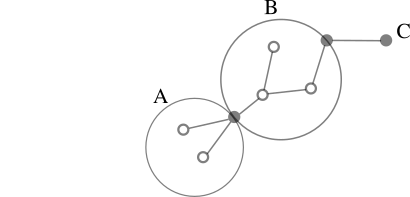
\includegraphics[scale=0.68]{02_dynamic_systems_and_control/png/network_schema}
% % \caption{Network Schema}
% % \label{fig:network_schema}
% % \end{figure}
% % 
% % Figure \ref{fig:network_schema} shows an inter-network with three networks \verb|A|, \verb|B| and
% % \verb|C|. The networks are connected with gateways marked as open circles. The endpoints are marked
% % as closed circles. Two gateways \verb|AB| and \verb|BC| are external gateways that interface between
% % two networks. All other open circles are internal gateways. Internal gateways are only required to
% % understand properties of their own network and also IP. External gateways are only required to
% % understand the properties of the two networks they interface with and also IP. There are no
% % requirement that gateways understand TCP or any higher-level protocols. The result is that all
% % responsibility for TCP is passed to the endpoints.
% % 
% % This architecture gives a great deal of flexibility, because on the condition that a network
% % understands IP the characteristics of its internal network are isolated from the rest of the
% % network. It also makes plugging the new network into the inter-network much less complex.
% % 
% % The problem with this design is that it imposes strong constraints of the network as a feedback
% % control system.
% % 
% % Components in the system have to satisfy network level requirements, but the system was designed to
% % strictly minimize the requirements of the gateways.
% 
% % TODO: There was a lot of discussion about what 'endpoint' meant.
% % TODO: It would have been possible to add congestion information transmission to the gateways, but
% % see Jacobson's story about Postel. Also at the time of design, gateways were an expensive
% % component in the system, and it wasn't clear at all that congestion would become a problem. 
% 
% % TODO: Common pattern in software engineering. The practical approach. Get the components working,
% % and then see later if the system works. Can't see into the future what problems will emerge.
% 
% % TODO: The important point is that the system doesn't work without a feedback protocol sitting on
% % top of IP. It doesn't need to be TCP. But it needs to be responsible for congestion control. The
% % connectionless packet idea (IP) is the component that is required of the gateways to know.
% 
% % The question is whether the endpoints need extra requirements in IP to send information to the TCP
% % level, so as to handle system requirements.
% 
% % TODO: But from the point of view of system design, it
% % should have been clear that there was a
% % problem, to ignore system requirements.
% 
% % TODO: This should go earlier in the Cyclades section. 
% 
% % This system is feed-forward. The protocol has no mechanism for the sending endpoint to learn
% % anything about the receiving protocol. But the network is a limited resource. Each link requires
% % time to transmit packets, and each gateway requires time to transmit and has a limited buffer for
% % storing queued packets waiting to be re-transmitted. 'best-effort' means that the sending end-point,
% % by using the IP protocol, can learn nothing about whether the receiving end-point received the
% % message, or the condition of the links and gateways on the route that was used. 
% % 
% % The TCP protocol is designed as a communication protocol between endpoints. Due to the requirement
% % to hide networks, it was designed to work by communication with its other endpoint, called its peer.
% % 
% % To satisfy the network, i.e. to share out its use fairly and to prevent congestion, the sending peer
% % is required to get its feedback response only from information received by the
% % 
% % This limits the amount of information that
% 
% % TODO sharing schema
% 
% % TODO layering schema
% 
% 
% % chapter:          Dynamic Systems
% % section:          Internet
% % subsection:       TCP/IP
% % subsubsection:    Control System Components
% % \subsubsection{Control System Components}
% % 
% % \begin{figure}[H]
% % \centering
% % \includegraphics[scale=0.28]{01_introduction/png/feedback_schema}
% % \caption{Control System Schema}
% % \label{fig:feedback_schema}
% % \end{figure}
% 
% % chapter:          Dynamic Systems
% % section:          Internet
% % subsection:       Congestion
% % \subsection{Congestion}
% 
% % chapter:          Dynamic Systems
% % section:          Internet
% % subsection:       Congestion
% % subsubsection:    TCP Feedback schema 
% % \subsubsection{TCP Feedback Schema} 
% 
% % \begin{quote}
% % By means of simulating TCP/IP network operations we are able to examine in detail the causes of
% % traffic oscillation in a simple network setting. Our analysis shows that users' control actions
% % are highly synchronized by the network congestion signaling and that providing users only a
% %     binary network state can lead to repeated oscillations\cite{zhang1990}.
% % \end{quote}
% 
% 
% % TODO: Check references [Leland94], [Flo94], [Zha90].
% 
% % chapter:          Dynamic Systems
% % section:          Internet
% % subsection:       Congestion
% % subsubsection:    The Actual Design
% % \subsection{The Actual Design}
% 
% % TODO: Place this image in the correct place
% 
% % \begin{figure}[H]
% % 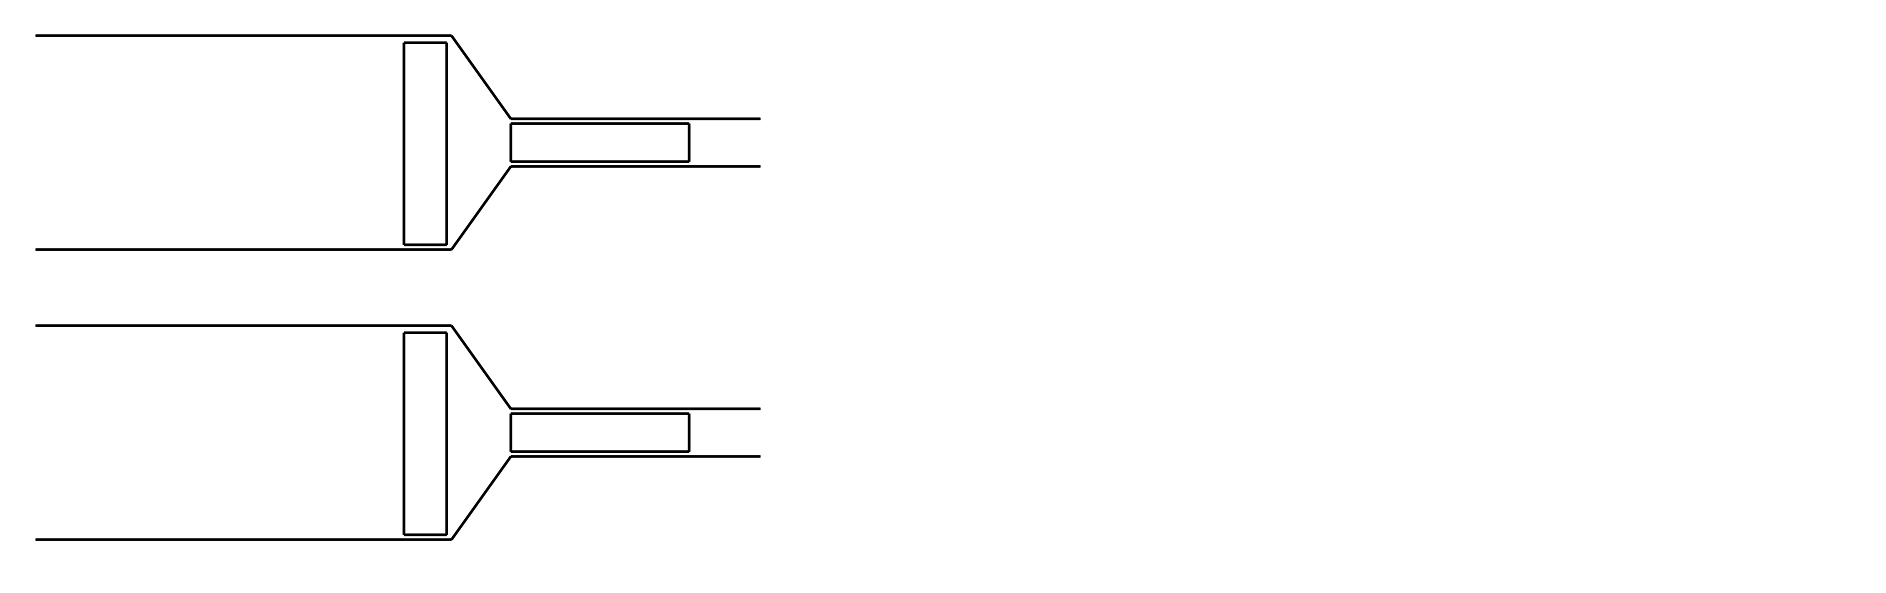
\includegraphics[scale=0.48]{02_dynamic_systems_and_control/png/bandwidth_transition}
% % \caption{Packets reaching bandwith transition}
% % \label{fig:bandwidth_transition}
% % \end{figure}
% 
% % ACK clocking is pseudo-mechanical. When this system was designed the cost (monetary and in time)
% % of computer processing was large. The IMP (the interface 'card') had 12K of memory and a cost of
% % hundreds of thousands of dollars. The ingenuity of mechanical feedback stabilization mechanism is
% % remarkable, and given the costs at the time, made sense. In general though, mechanical feedback
% % processes are highly inflexible (hence the ingenuity required) compared to a simple PID
% % controller.   
% 
% % What the actual design looked like
% 
% % The problem that occurred
% 
% % TODO: Describe the actual events that occurred.
% 
% % chapter:          Dynamic Systems
% % section:          Internet
% % subsection:       Congestion
% % subsubsection:    Congestion Events
% % \subsubsection{Congestion Events}
% 
% 
% % Thinking about the problem as a positive feedback
% 
% % chapter:          Dynamic Systems
% % section:          Internet
% % subsection:       Congestion
% % subsubsection:    Positive Feedback 
% % \subsubsection{Positive Feedback}
% 
% 
% % chapter:          Dynamic Systems
% % section:          Internet
% % subsection:       Routing
% % \subsection{Routing}
% 
% % \subsubsection{IP vs TCP}
% 
% % From a control system point of view, IP and TCP are separate. IP is fundamentally static. Packets
% % are set onto the network, and no measurement or response is taken. TCP is a dynamic process -
% % sending packets onto the network, collecting data from the network, and using that data to respond
% % to failures.
% % 
% % European method was IP, US approach was a combination of IP and TCP. In around 1978, the US team
% % separated out the (clearly different functionality from a control system point of view) IP and TCP.
% % 
% % \subsubsection{Dropping Packets}
% % 
% % Using dropped packets as a error measurement is problematic.
% % 
% % \subsubsection{Introduction to the Internet}
% % 
% % Our goal is to examine the different negative and positive feedback systems in the internet. How
% % important are these feedbacks to the design of the internet? What are the constraints on the design
% % of these feedbacks? Identify which designs have successfully solves problems, and which have not.
% % 
% % In general feedback design is embedded in algorithms and not so explicit, but are central to network
% % design from the beginning. 
% % 
% % \subsubsection{Cost}
% % 
% % Telephone networks have serial connections, meaning that failure in any link results in failure of
% % the connection. In consequence every link has to be very high reliability and therefore costly.
% % Packet switching networks could work across cheap wires and use software design to solve reliability
% % problems.
% % 
% % \subsubsection{Downsides}
% % 
% % The downsides of packet switching is the requirement for computing power and memory buffers and the
% % ends of network links.
% % 
% % \subsubsection{Social Resistance}
% % 
% % Roberts\cite{roberts1978} later reflected on the development of packet switching,
% % 
% % \begin{quote}
% % The very fact that no technological breakthrough was required to implement packet switching was
% % another factor weighing against its acceptance by the engineering community. What was required was a
% % total reevaluation of the performance and economics of dynamic-allocation systems, and their
% % application to an entirely different task. Thus, it remained for outsiders to the communications
% % industry, computer professionals, to develop packet switching in response to a problem for which the
% %     needed a better answer: communicating data to and from computers.
% % \end{quote}
% 
% % One might expect that the choice of route is determined by feeding back to the routing control
% % components in the system, information about round-trip times.
% % 
% % Very interestingly, this isn't how choice of route is determined.
% % 
% % In general, route choice is determined statically by the system administrators for each owned
% % component of network.  
% % 
% % This seems surprising on two points,
% % 
% % \begin{enumerate}
% %     \item If route choice is so static how can the system respond to change?
% %     \item Routes remain very dynamic. If we use 'traceroute' on an internet request, the route is
% %         always changing.
% % \end{enumerate}
% % 
% % The important point is that computer networks are extremely bursty and unpredictable. It is the
% % nature of computer network traffic that it occurs in bursts. This introduces large amounts of noise
% % into the feedback process. 
% % 
% % The way to handle this unpredictability is to increase the time-frame response. By aggregating data
% % we can smooth out the response. In other words, by making the feedback slower we can increase its
% % effectiveness.   
% % 
% % The companies that own the network are motivated to optimizing the this feedback process. So
% % economics comes into the loop.
% % 
% % One draw-back of economic feedback across the network is that system administrators optimize the
% % network for their own customers.
% % 
% % How does this guarantee that the network is also optimized for temporary non-paying users of that
% % network?
% % 
% % 
% % 
% % There are a couple of important economic lessons/analogies here:
% % 
% % 1. aggregating    
% % 2. feedback doesn't necessarily have to be built in from the smallest granularity upwards,
% %    system-administration of internet areas is sufficient.
% % 
% % It may well be (though not guaranteed) that the feedback in aggregated systems (such as the whole
% % economy) can work well, even if the components are clumpy (as in administrative areas in the
% % internet). [reword]
% % 
% % It is not a-priory guaranteed that such systems are stable or unstable. Ultimately, the stability of
% % a system can only be guaranteed through a process of redesign and testing (i.e. a scientific
% % process).
% % 
% % This is also experienced with the internet - we can see that iterative improvement process at all
% % levels, and redesign responses to failure.
% 
% % [history of fixing the problems of the internet]
% 
% 
% \subsection{Discrete Model}

    \section{Exchange Transactions}
\label{section:exchange_transactions}

% \subsection{Markets}

% One effort to explain the sustained failure or markets to equilibriate at the aggregate level is to
% try to explain failure of equilibriation as a result of the way individual economic behaviour
% aggregates to failure or otherwise of markets for single products to equilibriate, and further to
% explain failure of markets to equilibriate at the aggregate level.
% 
% A fundamental method of science and engineering is to assume as a first step, is to use the mean
% value to aggregate a collection of micro-level behaviours. Often this turns out not to be correct,
% but invariably, in virtually every system we seek to explain, there are some parts of the system we
% explain away by averaging out noisy behaviour. 
% 
% If we use the same technique for understanding economic behaviour, we would, as a first step assume
% that we can average markets for single goods or services, result in an aggregate supply or demand
% close to zero.
% 
% If we use the same technique for understanding economic behaviour, we would, as a first step assume
% that we can aggregate our model of supply and demand for single goods or services, and arrive at a
% aggregate where aggregate supply or demand is close to zero.
% 
% Since this conclusion is contrary to facts, economists have directed their efforts at modifying the
% supply and demand model in many ways in an effort to explain this contradiction between fact and
% theory.
% 
% What is clear, however, is that the explanation has to be sufficiently fundamental to explain the
% remarkably consistent fact of excess aggregate supply and the rarity of aggregate market
% equilibrium. As put forward by Lucas, economists have yet to find a convincing understanding of
% this fact, let alone to find a solution to the problem of equilibrium failure or the problem of
% a sustained positive unemployment rate. 
% 
% Since our explanation of these facts is outside is not a part of the supply and demand model, we
% assume our simplest model of market behaviour, and that markets at the aggregate level do in fact
% equilibriate, relying on the law of large averages.

\subsection{An Exchange Transaction Only Model}

We will start with a model simplified from Figure \ref{fig:economic_feedback_schema1}. that includes only
exchange transactions.

\begin{figure}[H]
\centering
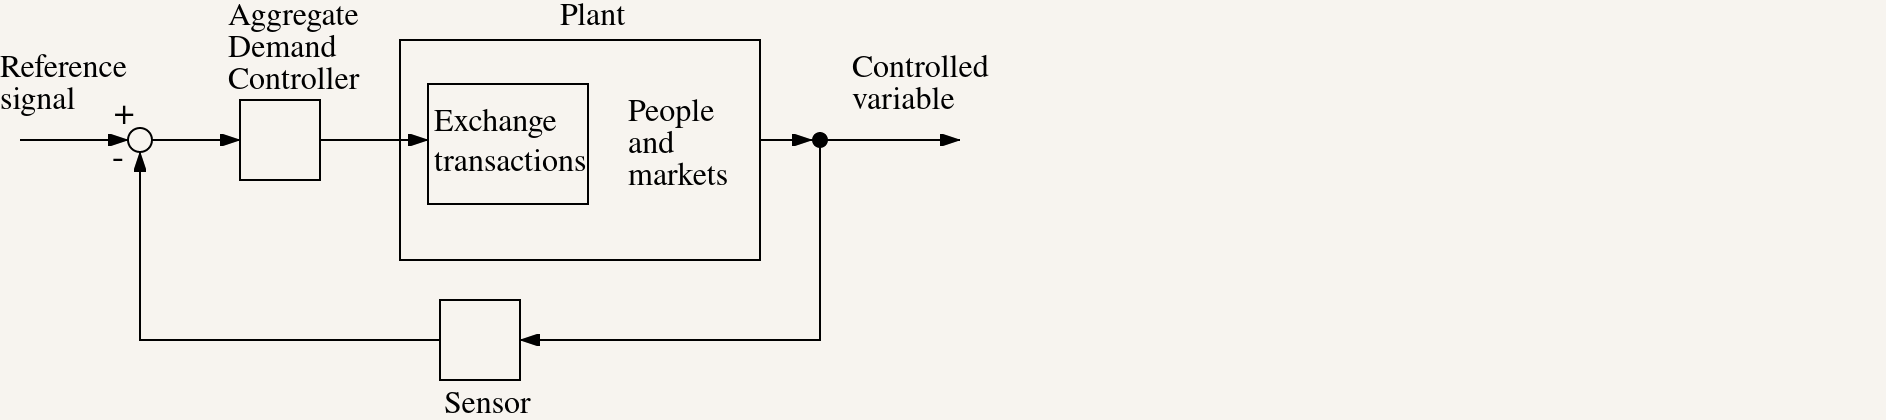
\includegraphics[scale=0.60]{03_exchange_transactions/png/exchange_only_feedback_schema}
\caption{Exchange Only Feedback Schema}
\label{fig:exchange_only_feedback_schema1}
\end{figure}

\subsection{Price and Quantity}

Starting with exchange transactions

\begin{figure}[H]
\centering
\includegraphics[scale=0.60]{03_exchange_transactions/png/exchange_transaction}
\caption{Exchange Transaction}
\label{fig:exchange_transaction2}
\end{figure}

we want to construct some aggregate variables. These aggregate variables could be sums, averages or
some other kind of measures of centrality. We'll categorize exchange transactions into different
``goods categories''. We'll use this term rather than say ``goods and services'' for brevity and
because it more closely reflects our requirements. We'll assume at this point that these goods
categories are sufficiently well-defined and precise as not to introduce too much noise into our
aggregate measures. For a given currency at a given period of time the transactions, we sum the
quantities for each goods category.

\[
    \left( q_1, \dots, q_N \right)
\]

and then let $pi$ be the average price of these transactions for a given good category. Let $N$ be
the total number of different goods categories. We'll denote the units for these values as

\[
    \left( \left[ q_1 \right], \dots, \left[ q_N \right] \right)
\]

We'll denote the average price for each $q_i$.

\[
    \left( p_1, \dots, p_N \right)
\]

The units for the average prices are 

\[
    \left( \left[ \frac {\$} {p_1} \right], \dots, \left[ \frac {\$} {p_N} \right]  \right)
\]

We cannot sum either these prices or quantities because they can have different units. But each
payment $p_i q_i$ can be summed because its unit, using dimensional analysis, is

\[
    \left[ \frac {\$} {q_i} \right] \left[ q_i \right] = \left[ \$ \right]
\]

So for a given time period, total payments for transactions for a currency is 

\[
    F = p_i q_i + \dots + p_N q_N
\]

We want to construct a aggregate measure of prices. As will become clear later in the paper we want
a measure $P$ that can be used to isolate purchasing power from the inflation rate. For example, if
a person has a certain amount of currency in their account at time $t=0$, and that they can buy a
certain amount with this currency, we want to know how much money they must have in their account at
time $t=1$ so that they can buy the same amount. As written, the notion of ``price level'',
``purchasing power'' and ``amount'' are vague and require mathematical treatment.

Suppose at a given time the transactions with quantites

\[
    \overline Q = \left( q_1, \dots, q_N \right) \textrm{ with corresponding prices } \left( p_1, \dots, p_N \right)
\]

occurs. We'll introduce Alice. We'll feed Alice a 1 dollar and Alice will spend this 1 dollar by
randomly selecting goods categories in such a way that in the limit they purchase quantities all in
proportion to total transactions. In other words,

\[
    \varepsilon_{q_1,\dots,q_n} = c_1 \overline Q
\]

where $c_1$ is a number between $0$ and $1$ and $\varepsilon_{q_1,\dots,q_n}$ is the expected value of
the ``abstract person'''s purchases. The $c_1$ represents the purchasing power of the Alice. It
represents the proportion of all transactions over which Alice has the power to purchase, per
dollar. While purchasing power is the amount of goods that will buy a given unit of currency, the
price level is its reciprocal, the amount of currency that will buy a unit of quantity.

We need to make things more precise, and to check that our measure of price can be used as an index
to isolate Alice's purchasing power from changes in the inflation rate. The motivate for this will
become clear later in the paper.

First we'll do a static analysis, and try to construct meaningful measures of aggregate price and
quantity for a time period that has 

\[
    \overline Q = \left( q_1, \dots, q_N \right) \textrm{ with corresponding prices } \left( p_1, \dots, p_N \right)
\]

Here, the vector $\overline Q$ represents a collection of values, but we want to construct a single
value that is a aggregate of these values. The problem is that each of these values may have
different units. We can construct units that such as ``one apple and two oranges''. The problem is
that if we do this it is impossible to express ``two apples and two oranges'' in these units. But if
we consider only a single period of time that has $\overline Q$ transactions, then we can express
this value in any unit of the form

\begin{equation}\label{equation:basket}
    \left( \left[ \gamma q_1 \right], \dots \left[ \gamma q_N \right] \right)
\end{equation}

for any number $\gamma$. So in fact there is not just one, but a set of feasible units in which to
express $\overline Q$. We refer to any one of these set of units as a ``basket of goods''. Given
that we select one of these sets of units, we can then express $\overline Q$ as some number $Q$,
where the units given by equation (\ref{equation:basket}) with a specific $\gamma$. The units of
$Q$ is this basket of goods. Now we can set the price level as the payment for this basket of goods.
This value $P$ is in units \$ per basket. And so

\[
    F = PQ
\]

The units used depends on the $\overline Q$ at a point in time. Of the proportion of $q_i$ changes
we would have to use a different unit, and so we couldn't do any dynamic analysis (comparisions
across time). We can solve this problem by further constraining our units. As noted, for any
$\overline Q$ at any time we can construct a new unit. We further constrain this by setting the rule
that given one basket of goods whose value of $\gamma$ is arbitrarily chosen, we constrain all other
baskets of goods, by setting their $\gamma$ to a value such that all baskets of goods have the same  
average of quantities weighted by their share of trade.

\[
    \frac 1 {\gamma} \left[ q_i \left( \frac {f_i} F \right) + \cdots + q_n \left( \frac {f_N} F
    \right) \right] = \frac 1 {\gamma'} \left[ q_i' \left( \frac {f_i'} {F'} \right) + \cdots + q_n'
    \left( \frac {f_N'} {F'}
    \right) \right]
\]

Now, because $\gamma$ depends only the trade-weighted average of $\overline Q$, the distribution of
$q_i$ around this average becomes irrelevant. This means that \textit{however} $\overline Q$
changes, whatever its distribution, the relation $F=PQ$ is exact.  














\subsection{Control of Price Level}

Before examining exchange transactions, we will briefly consider the feedback control mechanism.
Indexation is an important method for controlling distributed systems like a currency. An index is a
single value that is utilized by multiple components. An example of indexation in digital currencies
is Bitcoin's method for regulating the rate of production of blocks by Bitcoin miners. In this case
the indexation is algorithmic rather than controlled by a central authority. TODO

Another example of indexation is 

The simplest way to control the price level in a digital currency is to use indexation.





TODO

The feedback control loop does not work, however, in legacy currencies because the core currency
doesn't account for all money. Most money in legacy currencies is banking money, termed M1, M2 and
M3. Under these conditions, money authorities must use alternative methods to try and induce
financial institutions to increase the amount of banking money mainly through changing the interest
rate at which the money authority lends core currency to those financial institutions. At times this
method has been effective at controlling the price level, at other times less so. The process lacks
precision and has a long time-lag, making its use as the main mechanism for controlling economic
conditions problematic. Its effectiveness is also determined by financial institution's ability and
willingness to respond to decreases or increases in the monetary authority's core lending rate in a
way the maps to increases or decreases in aggregate demand.

\subsection{Market Symmetry}

    \section{Exchange Transactions and Errors}
\label{section:exchange_transactions_and_errors}

% A back-of-an-envelope calculation reveals that within an order of magnitude this hypothesis results
% in all the variables reacting with each other within an orderin a way we have observed in economic
% systems. An error rate of 5 percent is maybe reasonable. An error rate of 10 percent seems
% unreasonably large. From personal experience visiting a supermarket, there is some chance that a
% line of goods we were expecting to buy is not available. This is probably less than 1 in every 10
% purchases we are expecting to make. On the other hand 1 percent probably seems too small, though not
% impossible. Communication systems typically require 2.5 - 10 times the error rate to expend to
% compensate for errors, so we could assume a reasonable number is 5. The hypothesis implies that an
% increase in the growth rate  1 percent increase in the growth rate will cause a 1 in 5 percent
% increase the unemployment rate for a given inflation rate. This is certainly in the right direction
% but seems a little small. Unemployment rates typically fluctuate between 3 and 10 percent, but to
% drive a reduction in the unemployment rate from 10 percent to 3 percent would would require 35
% percent increase in the growth rate (with fixed inflation rate), which seems excessive. Nevertheless
% there is no variable that is reacting in an unexpected direction.
% 
% Given our rough numbers above, an increase of 5 percent in the inflation rate with a fixed growth
% rate, would result in a 1 percent reduction in the unemployment rate. This is certainly in line with
% the two most prominent economic papers on the relationship between the inflation rate and the
% unemployment rate, firstly Phillips and secondly Lucas.
% 
% TODO: Phillips figure and Lucas figure 

\subsection{Information Theory}

\begin{figure}[H]
\centering
\includegraphics[scale=0.48]{04_exchange_transactions_and_errors/png/error_intuition}
\caption{Intuition about Error Rates}
\label{fig:error_intuition}
\end{figure}

Intuitively we might think about how adding redundancy to a message might change the error rate as
in Figure \ref{fig:error_intuition}. The original message with a certain error rate and no
redundancy is represented by point $A$. If we add some redundancy to the error message we might be
able to reduce the error rate of the received message to $B$. It seems that the problem is that for
each piece of redundancy we add to the message, we introduce more errors, and so as we increase
redundancy we would get decreasing returns on improved error rate. Claude Shannon proved
mathematically that this intuition is incorrect, and that there exists a method of adding redundancy
to our message such that if we add a $H$ rate of redundancy we can remove all errors from the
message. The correct bound on the possible error rate is show in Figure \ref{fig:shannons_proof}.

\begin{figure}[H]
\centering
\includegraphics[scale=0.48]{04_exchange_transactions_and_errors/png/shannons_proof}
\caption{Shannon's Theorem of Noisy Channels}
\label{fig:shannons_proof}
\end{figure}

The value $H$ indicates the extra length required of a message so as to compensate for all messages.
It is determined by the probabilistic properties of the sent messages. We look into this in more
details in \ref{appendix:information_theory}.

\subsection{Aggregate Supply and Demand}
\label{section:aggregate_supply_and_demand_with_noise}

In Section \ref{section:aggregate_supply_and_demand} we presented a simple dynamic model of aggregate supply and
demand. For any engineering system we must handle the effects of errors or noise on the system. In
this section we will look at the effects of an error rate that reduces the per period aggregate
agreements of an economy to the actual transactions that eventuate in that period.

\begin{figure}[H]
\centering
\includegraphics[scale=0.48]{04_exchange_transactions_and_errors/png/ad_as_errors}
\caption{Unemployment as a Function of Aggregate Supply and Demand}
\label{fig:ad_as_errors}
\end{figure}

\underline{Case A. $AD=AS$ equilibrium}

In this case the level of agreements, measured in $\$$ is equal to aggregate supply and aggregate
supply. There is no  

\underline{Case B. Excess $AS$}

\underline{Case C. Small excess $AD$}

\underline{Case D. Large excess $AD$}

We enumerated four cases above, but we can think about this more abstractly, as each $\$$ being a
carrier for a message. We don't need to quantify the amount of information each unit of currency
carries. We do need to know what the relative reduction in that quantity is as it is `transmitted'
across the economy. So currency can be thought of as a carrier of economic information that is
distributed across the economy, and that its capability of reducing the error rate in this
transmission process is dependent on providing redundancy through increases in aggregate amount of
currency.

Whatever way we think about the problem, we can use Figure \label{fig:shannons_proof}. to determine the
increase in $F$ required. The physical bound on market interactions is therefore shown in the Figure
below. Case A, C and D are represented on the graph.

\begin{figure}[H]
\centering

\includegraphics[scale=0.48]{blank}
\caption{}
\label{fig:physical_bound}
\end{figure}



\subsection{Conclusion}

The design of systems generally require an interaction between many micro-level components and
macro-conditions. A well-designed system will meet certain macro-level conditions without overly
constraining micro-conditions. The macro-level conditions that a currency should aim for are
sustained and stable market equilibriation. We have shown that this condition is only met if a
level of inflation greater than entropy $H$ is maintained. This requires a unit of prices that is
constantly changing. The notion that the properties of the units used in a system affecting real
outcomes such as aggregate quantity of output $Q$ is unintuitive. We have now been able to shed
light on David Hume's problem. His question was why changing units of price should have any affect
real quantities. We have now come, at least part-way to solving this problem. However, as we
introduce more kinds of transactions into our system, we will find more challenges to the design of
a currency that will result in sustained and stable market equilibriation.  


    \section{Time Transactions}
\label{section:time_transactions}

\begin{figure}[H]
\centering
\includegraphics[scale=0.60]{05_time_transactions/png/time_transaction}
\caption{Time Transactions}
\label{fig:time_transactions2}
\end{figure}

\subsection{Including Time Transactions in Our Model}

\begin{figure}[H]
\centering
\includegraphics[scale=0.60]{05_time_transactions/png/time_transaction_feedback_schema}
\caption{Exchange and Time Transaction Feedback Schema}
\label{fig:exchange_and_time_transaction_schema1}
\end{figure}

In Section \ref{section:exchange_transactions_and_errors} we showed that there is a bound on the set of
economic transactions that are possible, and that the error bound is determined by $H$ (which we can
consider as beyond out control), the inflation rate $I$ and the growth rate $G$. We can control the
inflation rate, but in general the growth rate is external to our control. We also showed that to
achieve the goals of our currency requires a positive inflation rate. The unit in which we write
prices is continuously changing. The unit used to denominate payments in contracts is generally this
price unit. We show that this method of choosing interest rates is underspecified as discussed in
Section \ref{section:system_specification} such that under conditions of a positive rate of change
in the inflation rate, i.e. when

\[
    \frac {\Delta I} I > 0
\]

then either the real costs of borrowing must increase or the output $Q$ must decrease. Based on   
Figure \ref{fig:ui_bound} this results in unemployment/inflation tracking that appears as indicated
in Figure \ref{fig:underspecification_problem}.

\begin{figure}[H]
\centering

\includegraphics[scale=0.48]{blank}
\caption{Underspecification Tracking}
\label{fig:underspecification_problem}
\end{figure}

Unspecification tracking occurs until the rate of change in the inflation rate drops to zero or
becomes negative. The combination of the error bound and underspecification tracking leads to a
fundamental control problem. To set conditions where aggregate equilibrium is possible, the
inflation rate must be increased to region $D$ as shown in Figure \ref{fig:ui_bound}. As the
inflation rate increases, underspecification tracking reduces the growth rate, increases the
unemployment rate. The solution to this problem is to correct the units in which contracts are
written. If a unit of account of constant value is used, real interest rates can be trivially
specified because the unit directly measures real payments and so fully specifies our control
problem. Given that a currency limits transactions to exchange transactions and time transactions,
and that a unit of account of constant value is used, and given that there are no other unforseen
destabilizing effects, the currency can be controlled to maintain aggregate equilibrium. If a unit
of account of constant value is not used, it is not possible for a currency to maintain aggregate
equilibrium.

\subsection{Unspecification Problem}

We showed in Section \ref{section:exchange_transactions_and_errors}. that the unit in which prices are
denominated must be continuously changing.

\begin{figure}[H]
\centering
\includegraphics[scale=0.48]{05_time_transactions/png/time_transaction}
\caption{Time Transactions}
\label{fig:time_transaction_contracts}
\end{figure}

This unit is used in time transactions to denominate the initial lending of currency, to denominate
the repayment, and it is also common practice to use it to specify the repayment in a contract.
Because this unit in continuously changing, the value written into contracts must be written in such
a way as to specify a real interest rate, i.e. an interest rate written in terms of purchasing
power. Fisher \cite{fisher1907} notes that in order to specify a real interest rate $r$ then the
value $i$ needs to be written into contracts, where

\[
    i = (1+r)(1+I)
\]

Whatever real interest rate $r$ lenders and borrows agree upon, its is possible to write the value
$i$ into contracts to achieve this outcome. For a given principle $k$ the repayment of the principal
is $k(1+I)$ and the repayment of interest on that principal is $k(1+I)(1+r)$, and so total the
repayment of both principle and interest is

\[
     k(1+r)(1+I) = k(1+I) + k(1+I)(1+r)
 \]

From the left-hand side of this equation we can see that the payment denominated in the unit of
currency increases at the same rate as the inflation rate. Figure \ref{fig:control_for_equil}.
illustrates that to maintain a market equilibriation set point we need a feedback regulator that
responds to deviations in the inflation rate from the set point.  Not only does the inflation rate
$I$ changes, the rate of change of the  inflation rate $ \Delta I / I $ changes. This
changes the requirement to control the real iterest rate from a single-variable control problem, to
a two variable specification problem.





    \chapter{Data}
\label{chapter:data}

    \section{Contract Transactions}
\label{section:contract_transactions}

\subsection{Mechanism}

\begin{figure}[H]
\centering
\includegraphics[scale=0.60]{07_contract_transactions/png/contract_transaction}
\caption{Contract Transactions}
\label{fig:contract_transaction}
\end{figure}

\subsection{Negative Feedback}

There are two money transfers in a contract transaction. The first is a transfer of money in
exchange for a good. As with time transactions, interest rates are prices and are subject to
excess supply/excess demand response.

\subsection{Positive Feedback}

A positive feedback can occur if people believe that they can resell something at a later time
with a higher price. This may increase demand rather than reduce it as in the negative feedback
case.  This can occur with both exchange transactions and time transactions if the price of a good
is increasing over time. We'll look at the proces in \ref{section:other_transactions}. Land and
precious metals sometimes behave like this. We'll look at the proces in
\ref{section:other_transactions}.
 
\subsection{Proxy Accounts}

Contract transactions can be used to construct proxy accounts such as bank accounts, that are
external to the accounts of the digital currency.

\begin{figure}[H]
\centering
\includegraphics[scale=0.48]{07_contract_transactions/png/proxy_accounts}
\caption{Proxy Accounts}
\label{fig:proxy_accounts}
\end{figure}

Proxy accounts work by transacting contractural obligations, and adjusting those credits and debts
without the need to complete all transactions in the original currency. 

Figure \ref{fig:mirror_proxy}, Part A, shows a standard between a standard digitial currency. Part B
shows the situation where account holders 1 and 2 have passed responsibility to the management of these
accounts to a bank. The banks own accounts in the digital currenct, and present account holders 1
and 2 with a dollar value written on a piece of paper or on a computer, written in the diagram as
\verb|"\$"|. When a transaction is made by these two account holders, the bank mirrors this
transaction in its digital currency accounts.

Part C shows the situation where bank 1 and bank 2 have many customers, and a single digital
currency account that exactly mirrors the aggregate values in all the 'accounts' that the bank
presents to the account holders. 

It might be possible (and in reality is generally possible) for banks to agree with each other to
redeem transactions rather than at the exact time of a transaction but over a certain period of
time, such as a day. If the behaviour of the transactions is random meaning that the aggregate flow
of transactions from bank 1 to bank 2 cancel out the aggregate flow of transactions from bank 2 to
bank 1 over that time period, then banks can use a ``fractional reserve system'' and reduce that
holdings of digital accounts, without any change in the circumstances of the bank account holders.
Under a fractional reserve system the flow of transactions through banking accounts can be an order
of magnitude greater than through the core digital currency accounts.

This process requires that banks utilize contract transactions between the banks, so that payments
are not settled exactly at the time of transaction, are repayed by the end of the period. Time
transactions cannot be used as time transactions require a flow of goods between the two parties. So
making part C more explicit, we have figure \ref{}.

\subsection{Control of Price Level}

As first discussed in Section \ref{subsection:control_of_price_level}. proxy accounts multiply the
supply of money, and introduce problems for the control of the price level. 

If there are not proxy accounts it is possible to directly control the total amount of currency
through an index mechanism.  

\begin{figure}[H]
\centering
\includegraphics[scale=0.48]{07_contract_transactions/png/demand_index}
\caption{Demand Index Mechanism}
\label{fig:demand_index}
\end{figure}

The payment index is set by the monetary authority or by algorithm, and is globally accessible.
Payment labelling and negotiation and agreements are done in dollars (\$). An account holds a base
value, which remains constant when there are no transactions. The account holder however sees the
dollar value of their account, which is constantly updated as the payment index changes. The dollar
value of an account is the produce of the payment index and the base value. The account receiving a
payment converts its value into a base value by dividing by the payment index and adding this value
to the accounts current base value. Account holders are generally unaware of the base value, and
observe a gradually changing dollar value, similar to the way a bank account appends interest
payments. All the conversion between base value and dollar value is done automatically by the
digital currency.

The monetary authority or algorithm increases or decreases the payment index in order to control
aggregate excess supply or aggregate excess demand. In the presence of proxy accounts this control
mechanism breaks down. Banking accounts become part of the set of all accounts that through market
decisions made by account holders determine aggregate properties of the currency. Traditionally,
monetary authorities try to control aggregate values by financial and banking regulations and
through what are known are open-market operations, in which monetary authorities try to influence
the degree to which banks have contractual obligations with each other by controlling the interest
rate at which they can borrow the core digital account currency. This methods has at times been
effective at controlling aggregate supply but at other times ineffective. In the absence of proxy
accounts, control of the currency through a payment index is direct and likely to be timely,
equitable and with high precision. Using this indexation, the tide rises all boats to exactly the
same degree. Given that markets remain in equilibriation, the proportional increase in purchasing
power is exactly equal to the proportional increase in the price level for every account holder.
There is no lag between an increase in the payment index and increase in dollar value in accounts.   

\subsection{Interaction with Time Transactions}

Interest rates in traditional economies are highly correlated as a result of market activity. A
rough working model is to think of an economy as having a single interest rate, qualified by
``risk''.  Both contract transactions and time transactions share this common interest rate. If the
interest rate on contract transactions increases due to a positive feedback, at some point
it will exceed the market interest rate for time transactions only, resulting in decreases in
productive investment through time transactions while investment in a positive feedback bubble is
occurring. The dynamics of these kinds of interactions are impossible to predict, both during a
positive feedback event and subsequent to the positive feedback event when it is likely that a
certain proportion of contracts from time and contract transactions default. In addition, contract
transactions are unlimited in complexity of contractural arrangements. It is not possible to create
control mechanisms to regulate instabilities that can occur as the result of the use of contract
transactions.

\subsection{Currency Design and Contract Transactions}

To achieve a stable and sustained macro-level equilibrium currencies should be designed to prevent
contract transactions for the following reasons: 

1. Time transactions can be used for most, possibly all, productive investment.

2. Contract transactions destability price level control.

3. Contract transactions can destabilize the interest rate which affects time transactions.

4. Positive feedback in contract transactions are the most common cause of financial bubbles and
crashes. 

    \section{External Transactions}
\label{section:external_transactions}

\begin{figure}[H]
\centering
\includegraphics[scale=0.48]{08_external_transactions/png/external_transactions}
\caption{External Transactions}
\label{fig:external_transactions}
\end{figure}

Figure \ref{fig:external_transactions} shows an external transaction. Without some extra form of
coordination, implemented by some additional accounts, the transaction as it stands in the figure
would be very difficult to coodinate. But it captures the important property of external
transactions, that across the market boundaries the exchange rate is the rate of payments in
currency $A$ as a ratio of the rate of payments in currency $B$.

\[
    X = \frac A  B
\]


where $X$ is the exchange rate and the unit is

\[
    \left[ \frac {\$} {yen} \right]
\]

Following our program, we'll look at how external transactions interact with other transaction
types.

\subsection{External Transactions and Exchange Transactions}

\begin{figure}[H]
\centering
\includegraphics[scale=0.48]{08_external_transactions/png/external_and_exchange_tx}
\caption{Interaction of External and Exchange Transactions}
\label{fig:external_and_exchange_tx}
\end{figure}

There is a negative feedback stabilizing process that brings the exchange rate into equilibrium with
the relative price levels of the two currencies. This process was described by Cassel
\cite{cassel1914} in 1914. If   

\[
    \frac {P_A} {P_B} > \frac A B
\]

the goods and services in currency $B$ are cheaper than goods and services in currency $A$, and so
exports of goods and services from $B$ to $A$ increase, and exports of goods and services from $A$
to $B$ decrease. This process continues until an equilibrium where

\[
    \frac {P_A} {P_B} \dot{=} \frac A B
\]

where $\dot{=}$ represents the equilibrium state.

\subsection{External Transactions and Time Transactions}

Because time transactions also involve the exchange of goods and services, time transactions also
contribute to the stabilization process described in the previous section. Repayments across the
external transaction market are determined in earlier periods from short term to long term
contracts, and therefore do not have the equilibriating ``power'' that exchange transactions do.
Interest rate differentials across the two currencies are liable to cause unpredictable disturbances
across the two currencies.

\subsection{External Transactions and Contract Transactions}

Contract transactions are only minimally connected to an initial exchange transactions, but can
involve multiple and continuing payments for changes in contract status. This proces is liable to
cause strong disturbances unrelated to the equilibriating process, and therefore are highly likely
to introduce disturbances to the exchange rate equilibriating process. Exchange rates across legacy
currencies that have floating exchange rates can and often do experience rapid fluctuations in
exchange rates.

\subsection{Control of External Exchange}

If only exchange transactions are allowed as external transactions the exchange rate should
equilibriate to the relative prices levels of the two currencies, otherwise know as purchasing power
parity. The introduction of contract transactions are highly likely to cause disturbances to both
currencies, making it difficult to maintain macro-equilibriation goals. Time transactions, represent
a middle-ground between contract and exchange transactions. 

    \section{Other Transactions}
\label{section:other_transactions}

If the price a good or service can be resold at a higher price then another form of transaction is
possible. This transaction can induce a positive feedback loop as an increase in prices over time
cause other economic participants to enter the market, further increasing prices. Often part or all
of the motivation for buying land or precious metals is to transact in this way. One method to
prevent or limit this positive feedback instability is to use a separate currency for certain
classes of goods category, for example to use a specific currency to real-estate transactions. By
doing this it is possible to fix the exchange rate between the two currencies as an index that
tracks the average increases in prices of real-estate. Then a conversion between the two currencies
compensates for average changes in the price of this good.


    \section{Implementation}
\label{section:implementation}

\underline{Abstraction Layer over Accounts}

To implement a currency design that does not constrain 


we need to reconsider the interaction between the micro-level, the economic participants and owners
of accounts, and the macro-level requirements.

The design strategy we take is to define the macro-level requirements and then to search for ways to
control the currency so that the currency is likely to map out to those macro-level requirements.   

We specify the macro-level requirements as

1. Sustained stability.

2. Macro-level equilibriation.

Simple accounts that hold a number with some control of the aggregate value in all accounts is the
digital equivalent of paper money. This design is insufficiently controlled to achieve our two
macro-level requirements.   

To achieve these outcomes we apply a abstraction layer over these accounts. This abstraction layer
does the following:

\underline{Exchange Transactions}

1. Present to the user a value that is the product of the user's base account value and an single,
global value that we call the demand index ($D_x$). This product is the value that users generally
see and is the value in which price agreements are made. This value gradually changes as the demand
index changes, appearing to users much as a bank account that has gradual increases as an interest
rate is applied to it. As such, it presents no usability difficulties to the user.

3. All exchange transactions must be associated with a quantity and a goods or service category. An
exchange transaction is only valid if both the seller and buyer confirm the same goods or service
category. This serves three purposes.

a. It asserts that the transaction is an exchange transaction, and as such, has no associated
contract with it beyond the current delivery of the goods or service. By doing this it confirms that
there are no future legal commitments to any future repayment. This is required to limit the use of
exchange transactions for the purpose of some other transaction category.

b. The data can be used, with necessary software mechanism to ensure the privacy of the data, to
accurately calculate the price index. 

c. It serves as a record for the seller and buyer to resolve any disputes, i.e. it acts as a
receipt or record of agreement.

Beyond the seller and buyer entering the same goods and service category, it is easy for seller and
buyer to collude and provide incorrect information.

4. There are intermediate accounts. These are required because all exchange transactions must be
associated

TODO

\underline{Time Transactions}

2. Values that set future payments, in particular for repayments on time transactions, are
denominated in a root value and the product of the price index ($P_x$). In this way, the purchasing
power of that value remains absolutely constant, and as such there it present any possibility of
inflation feedback. All repayments on time transactions must be defined at the time the money is
borrowed and designated as a time transaction.

\underline{Contract Transactions}

Contract transactions are prevented by the requirement that borrowers must make repayments to the
same party that initially lent the money. There are possible ways that users could subvert these
requirements which we discuss in a later section.

\underline{External Transactions}

The provision of an exchange transaction mechanism will be deferred. The possibility of providing
exchange transaction functionality with external currencies depends on the design of external
currencies, in particular the accuracy of their price index, and their control over contract
transactions. If we consider external transactions between two currencies of the kind we are
presenting in this paper, then an external exchange rate fixed to the relative price index of the
two currencies, and restricting transactions to exchange transactions by requiring the recording of
goods or service cateogry and quantity may be a suitable design. This kind of system would require a
pair of special aggregate accounts specifically for external transactions to pair up inflow and
outflow. In this system, the pairing of inflow and outflow would halt if either account became
empty. Another possibility would be to implement a floating exchange rate. The potential difficulty
with this design is that it is relatively easy for users to use exchange accounts in lieu or time or
contract transactions, and so it may be possible for users to engage in high-frequency capital
interactions across the external boundary despite the disincentive of having no legal resort on
repayment failure.

\underline{Usability}

The controls we plan to implement will have minimal impact on any user who intends to use the
currency for exchange or time transactions. There is an additional requirement for both seller and
buyer to agree on a transaction and to record goods category. Indexed units of account have been
used in Chile for a number of decades without significant usability problems, and the use of indexed
units of account in a digital currency could potentially further simplify their use.

One important exception, however, are restrictions on the types of repayment schedules for time
transactions. If repayment schedules are overly flexible, the repayments could possibly be used,
given people's ingenuity in using financial mechanisms to enrich themselves, as a substitute for
contract transactions. The extent to which this would happen in practice is unknown, and so starting
with relatively strict controls and relaxing restrictions with experience is probably a reasonable
approach.

\underline{Using One Transaction Category in Lieu of Another}

The are various methods that users may potentially use to one category of transaction of another.
The most serious risk is that users find ways to make contract transactions. The main barrier to
preventing this is to ensure that repayments can only be made to the initial lender's account. The
second barrier is to ensure that there is no legal protection to protect creditors from debtor's
failure to make ``repayments''. These barriers should be sufficient on the condition that there are
no significant economic incentives for engaging in such activity. In general such users will choose to
use other currencies, rather than a currency with these barriers.


    \section{Conclusion}
\label{section:conclusion}

We summarize the theoretical components according to the level of confidence in the results.

\underline{The error effect and Fisher lines}

This property is determined by physical properties and the inferences made from these rules are
sufficiently precise and measurable to be subject to falisification.

\underline{Aggregate equilibrium}

The property is an aggregate of people's behaviour that has been observed over long-periods or time with
great consistency and is a plausible outcome of people's general incentives. Our model remains
robust even if we relax this assumption to a large degree. Almost all fields of economic research
are predicated implicitly or otherwise on the idea that this condition must be modified heavily to
explain real-world conditions, and therefore require significant re-appraisal given that these
effects are better explained as a property of currency design.

\underline{Inflation feedback and financial bubbles and crashes}

These processes are best explained as positive feedbacks that, while their degree and timing cannot
be reasonable determined quanititatively with precision, if unchecked will have clear consequences
and these consequences have consistently observed. These positive feedback processes are
fundamentally uncontrollable with possible rapid changes that we cannot easily regulate. A
successful control system will strongly limit the impact of positive feedback processes.

\underline{Market driven changes in aggregate quantities and prices}

We cannot expect to be able to predict theses changes, but the rate of change is not sufficiently
fast that it cannot be controlled or adjusted for through feedback regulation.

We hope that this paper can lead to new directions in research. In all new engineering endeavours,
theory and practice diverge. We can take advantage of the relative easy of building digital
currencies to specific design specifications to make currency engineering into an experimental
science. Given the theoretical foundations presented in this paper there is a reasonable high chance
that we can design and build currencies that will not prevent markets from reaching equilibrium,
that that a stable equilibrium can be maintained indefinitely in response to changing conditions. 

    
\subsection{Endnotes}

According to Rathgeber's notes, the error effect was discovered in 1974. Rathgeber's papers glossed
over some matters that caused considerable confusion and doubt about the value of his work. I have
tried to make explicit those sources of ambiguity. Rathgeber discusses the need to separate out the
``functions of money''. This was a source of confusion and lack of precision, which I tried to deal
with using the notion of transactions as a way to delineate the different functions of money.
Rathgeber did not make a clear distinction between a currency as a technical property as compared
to the market behaviour of people, but the notion was implicit in his work.  This was also a source
a confusion, because people, quite reasonably, object to the application of engineering method
directly to social interaction. Making explicit the difference between markets and currency
hopefully clear that engineering method is applied to currencies, not social interaction. Rathgeber
was working in the context of a single, national, centralized currency. I have extended the
application of his ideas to digital currencies.  At the time he wrote his private papers, he had
access only to Australian inflation and unemployment data. I have extended this to data available up
to the time of publication.






    \begin{thebibliography}{9}

\bibitem{baran1964intro}
    Paul Baran,
    \emph{On Distributed Communcations: I. Introduction to Distributed Communications Networks}
    August 1964.

\bibitem{baran1964b}
    Sharla P. Boehm and Paul Baran,
    \emph{On Distributed Communications: II. Digital Simulation of Hot-Potato Routing in a Broadband
        Distributed Communications Network},
    August 1964.

\bibitem{baran1964c}
    Paul Baran,
    \emph{On Distributed Communications: IV. Priority, Precedence, and Overload},
    August 1964.

\bibitem{baran1964d}
    Paul Baran,
    \emph{On Distributed Communications: VII. Tentative Engineering Specifications and Preliminary
        Design for a High-Data Rate Distributed Network Switching Node},
    August 1964.

\bibitem{baran1964e}
    Paul Baran,
    \emph{On Distributed Communications: VIII. The Multiplexing Station},
    August 1964.

\bibitem{baran1964f}
    Paul Baran,
    \emph{On Distributed Communications: IX. Security, Secrecy and Tamper-Free Considerationgs},
    August 1964.

\bibitem{bennet1996}
    Stuart Bennet,
    \emph{A Brief History of Automatic Control},
    IEEE Control Systems Magazine,
    volume 16,
    issue 3,
    June 1996,
    pages 17-25,
    doi: 10.1109/37.506394.

\bibitem{cassel1914}
    Gustav Cassel,
    \emph{Money and Foreign Exchange After 1914},
    Macmillan,
    1923,
    p.137.

\bibitem{cerf1974}
    Vinton G. Cerf and Robert E. Kahn,
    \emph{A Protocol for Packet Network Intercommunication}.
    IEEE Transactions on Communications,
    volume 22,
    number 5,
    May 1974.

\bibitem{davies1966}
    D.W. Davies,
    \emph{Proposal for a Digital Communications Network},
    June 1966.

\bibitem{davies1967}
    D.W. Davies, K.A.Bartlett, R.A.Scantlebury, P.T.Wilkinson,
    \emph{A Digital Communications Network for Computers Giving Rapid Response at Remote Terminals}
    Proceedings of the ACM Symposium on Operating System Principles.
    1967.

\bibitem{feller1957}
    William Feller,
    \emph{An Introduction to Probability Theory and its Applications}
    John Wiley and Sons,
    1957.

\bibitem{fisher1926}
    Irving Fisher, 
    \emph{A Statistical Relation between Unemployment and Price Changes}
    International Labour Review,
    1926,
    volume 13,
    pages 496-502,
    1926.

\bibitem{fisher1907}
    Irving Fisher,
    \emph{The Rate of Interest},
    Macmillan Company,
    1907.

\bibitem{hamming1950}
    R.W.Hamming,
    \emph{Error Detecting and Error Correcting Codes},
    The Bell System Technical Journal,
    volume 14,
    number 2,
    April 1950,
    pages 147-160.

\bibitem{hughes1971}
    T.P.Hughes,
    \emph{Elmer Sperry: Inventor and Engineer}
    1971.

\bibitem{hume1741}
    David Hume,
    \emph{Of Money, Essays, Moral, Political and Literary},
    1741.

\bibitem{jacobson1988}
    Van Jacobson,
    \emph{Congestion Avoidance and Control},
    Proceedings of SIGCOMM 'ii
    August 1988.

\bibitem{kleinrock1978}
    Leonard Kleinrock,
    \emph{Principles and Lessons in Packet Communication},
    Proceedings of the IEEE,
    volume 66,
    number 11,
    November 1978.

\bibitem{leland1993}
    Will E. Leland, Murad S. Taqqu, Walter Willinger and Daniel V. Wilson,
    \emph{On the Self-Similar Nature of Ethernet Traffic},
    ACM SIGCOMM Computer Communication Review,
    volume 23,
    issue 4,
    October 1993.

\bibitem{lamport1977}
    Leslie Lamport,
    \emph{Proving the Correctness of Multiprocess Programs}
    IEEE Transactions of Software Engineering,
    volume SE-3,
    number 2,
    March 1977.

\bibitem{lucas1996}
    Robert E. Lucas Jr.,
    \emph{Nobel Lecture: Money Neutrality},
    The Journal of Political Economy,
    1996,
    volume 104,
    pages 661-682.

\bibitem{mackay2003}
    David J.S. MacKay,
    \emph{Information Theory, Inference, and Learning Algorithms},
    Cambridge University Press,
    2003.

\bibitem{paxson1995}
    Vern Paxson and Sally Floyd,
    \emph{Wide-Area Traffic: The Failure of Poisson Modeling},
    IEEE/ACM Transactions on Networking,
    June 1995.

\bibitem{phillips1958}
    A.W. Phillips,
    \emph{The Relation between Unemployment and the Rate of Change of Money Wage Rates in the United Kingdom, 1861-1957},
    Economica,
    1958,
    volume 25,
    pages 283-299.

\bibitem{rfc827}
    RFC 827,
    \emph{Exterior Gateway Protocol (EGP)},
    Eric C. Rosen,
    October 1982.

\bibitem{rfc896}
    RFC 896,
    \emph{Congestion Control in IP/TCP Internetworks},
    John Nagle,
    January 1984.

\bibitem{rfc7567}
    RFC 7567,
    \emph{IETF Recommendations Regarding Acrive Queue Management},
    F. Baker and G. Fairhurst,
    July 2015.

\bibitem{roberts1978}
    Lawrence Roberts,
    \emph{The Evolution of Packet Switching},
    Proceedings of the IEEE,
    December 1978.

\bibitem{shannon1945}
    Claude E. Shannon,
    \emph{Communication Theory of Secrecy Systems},
    1945,
    pages 84-143.

\bibitem{shannon1948}
    Claude E. Shannon,
    \emph{A Mathematical Theory of Communication},
    The Bell System Technical Journal,
    volume 27,
    pages 379-412,
    1948.

\bibitem{shiller1998}
    Robert J Shiller,
    \emph{Indexed Units of Account: Theory and Assessment of Historical Experience},
    NBER Working Paper Series,
    volume 6356,
    1998.

\bibitem{abildren2011}
    Kim Abildren and Jens Thomsen,
    \emph{A Tale of Two Danish Banking Crisis},
    Monetary Review,
    Danmarks Nationalbank,
    1st Quarter 2011,
    volume 1,

\bibitem{astrom2009}
    Karl Johan Astrom and Richard M. Murray,
    \emph{Feedback Systems: An Introduction for Scientists and Engineers},
    2009.

\bibitem{douglas2019}
    Brian Douglas,
    \emph{The Fundamentals of Control Theory},
    2019.

\bibitem{douglas1939}
    Paul H. Douglas et al,
    \emph{A Program for Monetary Reform},
    1939.

\bibitem{einaudi2006}
    Luigi Einaudi,
    \emph{The Theory of Imaginary Money from Charlemagne to the French Revolution},
    2006.

\bibitem{honkapohja2009}
    Seppo Honkapohja,
    \emph{The 1990's Financial Crises in Nordic Countries},
    Bank of Finland Research Discussion Papers,
    2009,
    volume 5.

\bibitem{jevons1876}
    William Stanley Jevons,
    \emph{Money and the Mechanism of Exchange},
    1876,
    chapter 25.

\bibitem{keynes1914}
    John Maynard Keynes,
    \emph{A Treatise on Money},
    1914,
    volume 1,
    chapter 1,
    Money and Money-of-Account.

\bibitem{keynes1936}
    John Maynard Keynes,
    \emph{The General Theory of Employment, Interest, and Money},
    1936.

\bibitem{lefort:2002}
    Fernando Lefort and Klaus Schmedt-Hebbel,
    \emph{Indexation, Inflation and Monetary Policy: An Overview},
    Central Bank of Chile,
    2002.

\bibitem{marshall1925}
    A.C. Pigou,
    \emph{Remedies for Fluctuations in General Prices},
    in Memorials of Alfred Marshall,
    1925.

\bibitem{maxwell1868}
    J. Clerk Maxwell,
    \emph{On Governors},
    March 5, 1968.

\bibitem{mill1848}
    John Stuart Mill,
    \emph{Principles of Political Economy},
    1848.

\bibitem{minorsky1922}
    Nicolas Minorsky,
    \emph{Directional Stability of Automatically Steered Bodies},
    Naval Engineers Journal,
    volume 32,
    issue number 2,
    1922.

\bibitem{mogul2005}
    Jeffrey C. Mogul,
    \emph{Emergent (Mis)behavior vs. Complex Software Systems},
    HP Laboratories,
    2005.

\bibitem{sperry1913}
    Elmer A. Sperry,
    \emph{Engineering Applications of the Gyroscope},
    Journal of the Franklin Institute,
    volume 175,
    Number 5,
    May 1913.

\bibitem{wescott2016}
    Tim Wescott,
    \emph{PID Without a PhD},
    2016.

\bibitem{wright1908}
    Orville and Wilbur Wright,
    \emph{The Wright Brothers Aeroplane},
    Century Magazine,
    September 1908.

\bibitem{zhang1986}
    Lixia Zhang,
    1986.

\bibitem{zhang1990}
    Lixia Zhang and David D. Clark,
    \emph{Oscillating Behavior of Network Traffic: A Case Study Simulation}
    Internetworking: Research and Experience,
    volume 1,
    pages 101-112,
    1990.

\end{thebibliography}



\end{document}

